%!TEX TS-program = xelatex
%!TEX encoding = UTF-8 Unicode

\documentclass[11pt,tikz,border=1]{standalone}
\usetikzlibrary{positioning}

\begin{document}
  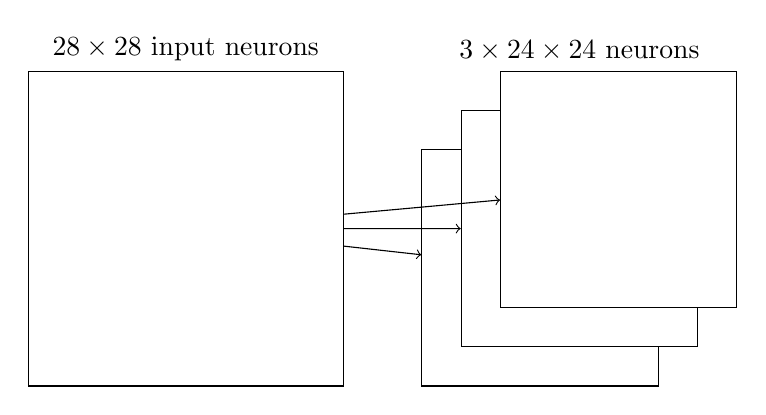
\begin{tikzpicture}[
    inputlayer/.style={rectangle,draw,fill=white,inner sep=0pt,minimum size=40mm},
    hiddenlayer/.style={rectangle,draw,fill=white,inner sep=0pt,minimum size=30mm}
    ]

    \node (input) [inputlayer,anchor=south west] at (0,0) {};

    \node (hidden0) [hiddenlayer,anchor=south west] at (5,0) {};

    \node (hidden1) [hiddenlayer,anchor=south west,xshift=5mm,yshift=5mm] at (hidden0.south west) {};

    \node (hidden2) [hiddenlayer,anchor=south west,xshift=5mm,yshift=5mm] at (hidden1.south west) {};

    \node [above] at (input.north) {$28 \times 28$ input neurons};
    \node [above,xshift=-5mm] at (hidden2.north) {
      $3 \times 24 \times 24$ neurons
    };

    \foreach \x in {0,...,2}
      \draw[->] (input) to (hidden\x);

  \end{tikzpicture} 
\end{document}
